\part{Verastegui}

\section{Introduction}

\section{Compression Consolidation}

\subsection{Stress State : Normalement consolidé ou surconsolidé}

\begin{figure}[h]
    \center
    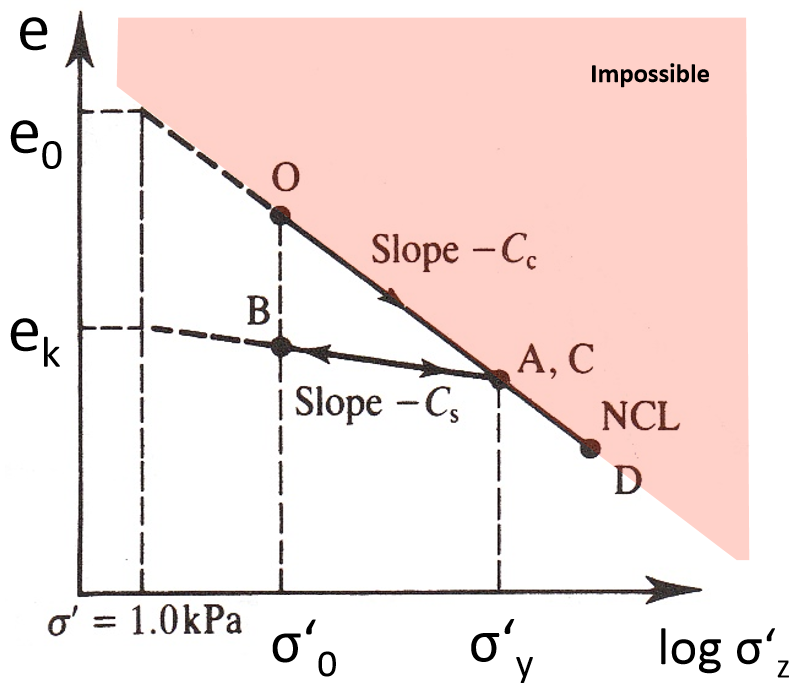
\includegraphics[scale=0.3]{Verastegui/images/V1.PNG}
\end{figure}

\begin{itemize}
    \item Le comportement du sol le long du segment NCL est élastoplastique.
    \item Le comportement du sol à la ligne de déchargement/rechargement est principalement élastique
    \item L'état de surconsolidation est caractérisé par un dégré de surconsolidation $R_p$ (
    $R_p =  NC$  si  $R_p > OC$)
\end{itemize}

\medskip

\begin{center}
\begin{tabular}{c|c}
    $R_p = \frac{P'_{yield}}{P'_0}$  &   $P'_{yield}$ = "yield" stress (pression de préconsolidation)  \\
      &  $P'_0$ = pression "actuelle"     
\end{tabular}
\end{center}

\subsection{Les effets du chargement}

Il y a un renfoncement $s$ qui se produit sur une période $t$. Cette période dépend de la perméabilité du matériau en présence, de la longueur du chemin de drainage et des conditions limites. Le sol se tasse en évacuant l'eau présente entre ses grains, donc un sol très perméable comme le sable se tassera plus vite qu'un sol argileux. 

\begin{figure}[h!]
\center
   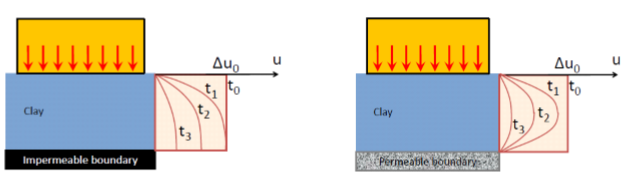
\includegraphics[scale=1]{Verastegui/images/V2.PNG}
\end{figure}

Ce phénomène est appelé consolidation.

\subsection{La théorie de la consolidation}

Pour la démonstration, voir slide 31 - 39 "Lesson\_Compr\_Consolidation"

\begin{multicols}{2}

    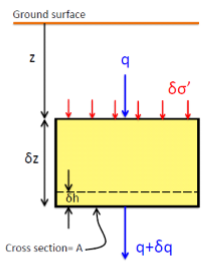
\includegraphics[scale=1]{Verastegui/images/V3.PNG}
    \vfill\null\columnbreak
    
    \begin{tabular}{|c}
         q: the inflow of pore water  \\
         q+$\delta q$: the outflow of pore water  \\
         $\delta z$: the heightof the differential soil element  \\
         $\delta h$: the deformation due to the load application  
    \end{tabular}

     
\end{multicols}


On y apprend que la consolidation du sol peut se calculer grâce à une équation différentielle. Dans un cas classique, à savoir une augmentation constante dans le temps de la force sur le sol, on peut la simplifier en une équation en une dimension. Celle-ci peut être finalement résolue numériquement ou par solution approchées.

\medskip

\begin{center}
\begin{tabular}{c|c}
    $u(z) = \sum_{m = 0}^{m = \infty} \frac{2 u_0}{M} (sin \frac{Mz}{H_{dr}}) e^{-M^2T_v}$ &   $ M = \frac{1}{2} \pi (2m + 1)$ \\
     &  $T_v = \frac{C_v t}{H_{dr}^{2}} $ "facteur de temps normalisé"
\end{tabular}
\end{center}

\medskip

Ces équations dépendent de la hauteur du sol $z$ et nous la voulons en fonction du temps. On utilise une approximation : 

\medskip
\begin{center}
\begin{tabular}{c|c}
    $S(t) = S_{inf} U(t) $ \quad &   $ U(t=\infty) =100\% $  \\
     &  $ U = \frac{A_{soil}}{A_{init}} $ 
\end{tabular}
\end{center}
\medskip 

On peut tout assembler pour estimer le degré de consolidation $U(t)$ avec l'équation : 

\medskip
\begin{center}
$ U(t) = 1 - \sum_{m = 0}^{m = \infty} \frac{2}{M^2} e^{-M^2T_v} $
\end{center}
\medskip

Finalement on trouve une autre approximation pour $T_v$, le facteur temporel normalisé :

\medskip 
\begin{center}
    $ T_v = \frac{\frac{\pi}{4} (\frac{U(\%)}{100})^2}{(1-(\frac{U(\%)}{100})^{5.6})^{0.357}} $
\end{center}
\subsection{Évaluation du coefficient de consolidation $C_v$}

    On calcule $T_v$ pour un degré de consolidation de x\% (ici de 50\%), on connaît une relation vue juste au-dessus qui lie $T_v$ à $C_v$. Il nous reste a évaluer $t_x$ (dans notre exemple $t_{50}$ ce qui correspond à $ U = 50\% $) pour avoir toutes les données nécessaires pour calculer $C_v$ (voir figure~\ref{fig:coefficient_consolidation}).
    
    \begin{figure}[ht]
        \begin{multicols}{2}
            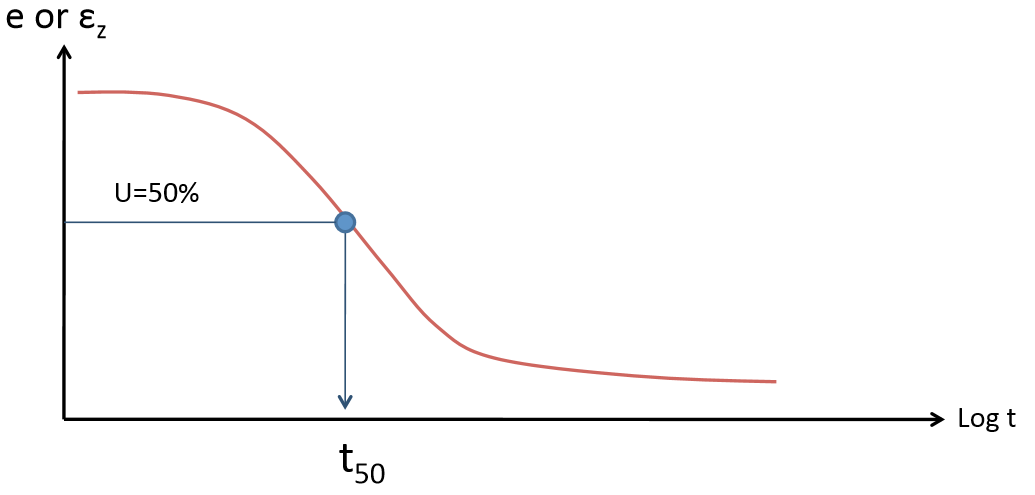
\includegraphics[width=\linewidth]{Verastegui/images/V4.PNG}
            \vfill\null\columnbreak
            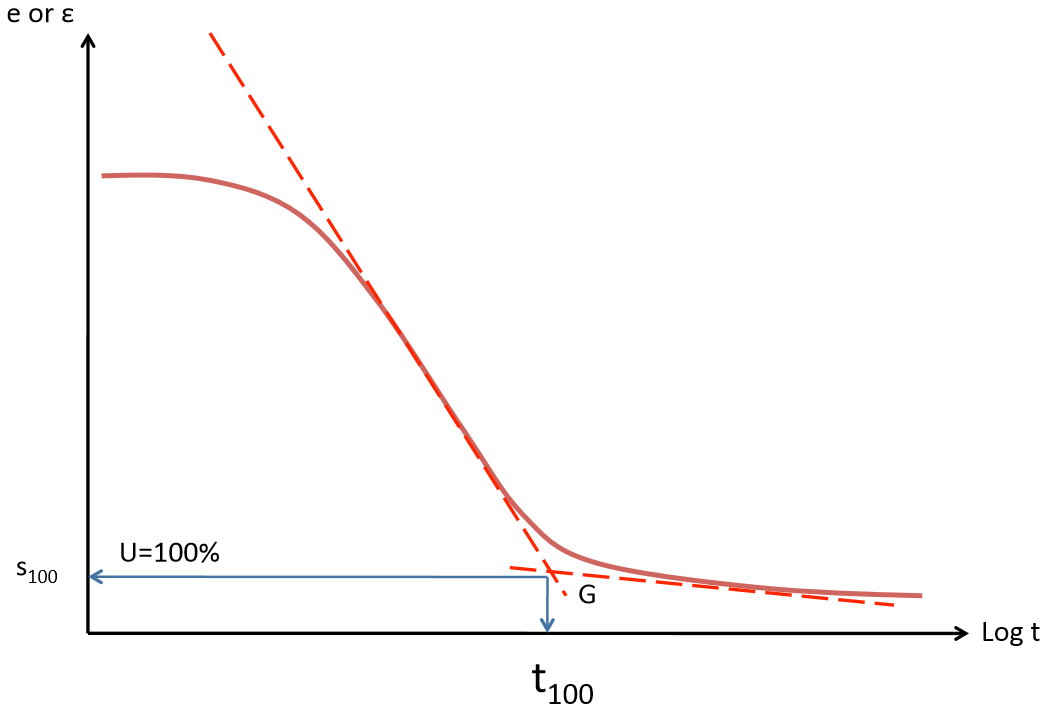
\includegraphics[width=\linewidth]{Verastegui/images/V5.PNG}
        \end{multicols}
        \caption{\'Evaluation du coefficient de consolidation}
        \label{fig:coefficient_consolidation}
    \end{figure}

    Attention à bien évaluer le temps $t_x$ sur le graphe. Pour $t_{100}$ il s'agit du croisement entre les deux tangentes des courbes représentatives. Pour $t_0$ c'est plus technique. Il faut placer deux points : P et Q dans la portion initiale de la courbe de manière à ce que $t_q = 4 t_p$. Trouver ensuite l'intersection E des droites parallèles aux axes passant par P et Q et faire la symétrie de E par rapport à P. Le point F ainsi trouvé aura le même indice des vides que notre cas $U = 0\%$. En regardant son point de croisement avec la tangente à la première courbe caractéristique, et en transposant ce point sur l'axe log t, on trouvera le point $t_0$. \\
    
    \begin{center}
    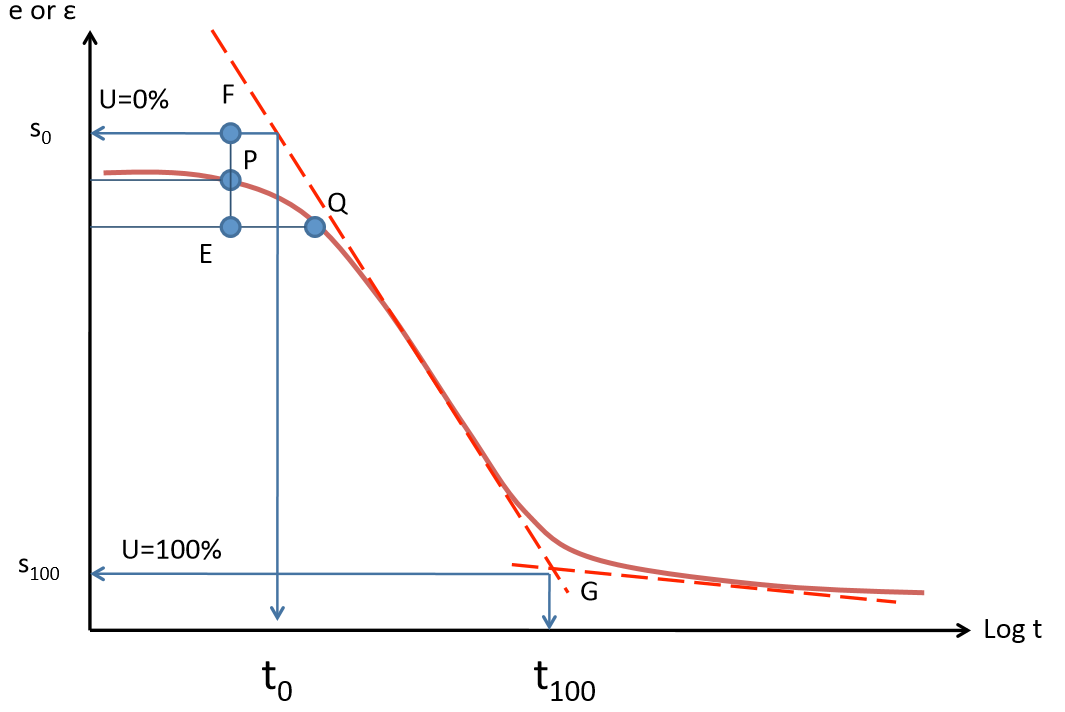
\includegraphics[scale=0.5]{Verastegui/images/V6.PNG} 
    \end{center}
    
\subsection{Compression secondaire}
    
    Une déformation naturelle du sol continue indéfiniment même après la consolidation. Ces déformations ne sont plus due à la dissipation de la pression intersticielle, mais au réarangement des particules. Dans les sols "mou" (soft), ces renfoncement peuvent être significatif. Cette déformation est observable dans le graphe ci-dessus, il s'agit de la deuxième courbe "commençant" lorsqu'il n'y a plus d'eau dans le sol ($S_100$). Cette compression se calcule grâçe à la formule suivante : \\
    
    \begin{center}
    \begin{tabular}{c|c}
    $ \rho_{sc} = \frac{H_0}{1+e_P} C_\alpha \log \frac{t}{t_p} $  &   $t_p = t_{100}$ temps de fin de la consolidation primaire  \\
        &  $H_0 = $ épaisseur en $t_{100}$ 
    \end{tabular}
    \end{center}
    
    Il existe des formules combinant les déformation de consolidation primaire et secondaire : 

    \begin{center}
    $S_t = H\Delta\sigma'(\alpha_p + \alpha_s \log t)$
    
    \smallskip
    $S_t = H(\frac{1}{C_{pr}} + \frac{1}{C_{sec}} \log t) \ln \frac{\sigma'_i + \Delta \sigma'}{\sigma'_i}$
    \end{center} 
    
\section{Mohr Circles}

    \begin{multicols}{2}
        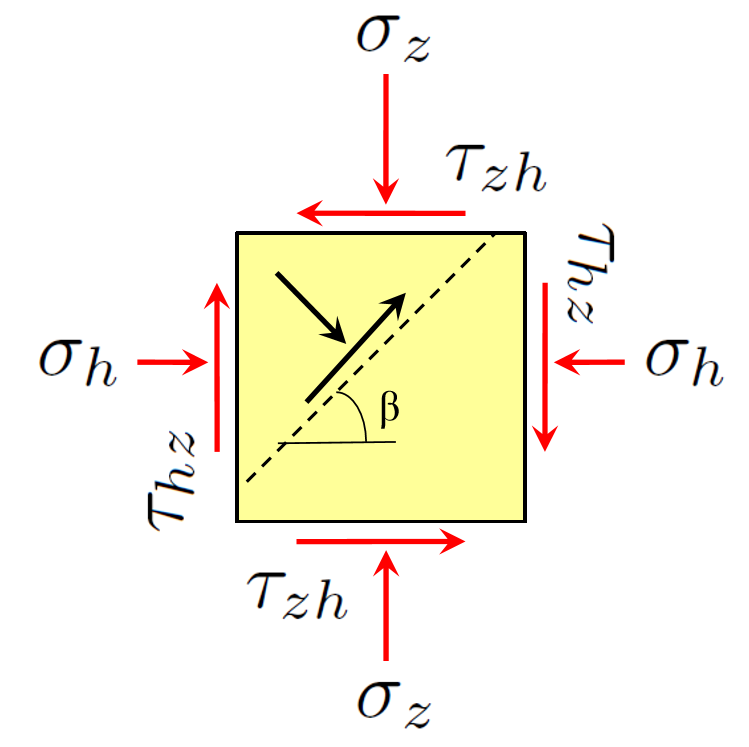
\includegraphics[scale=0.4]{Verastegui/images/V7.PNG} \\
        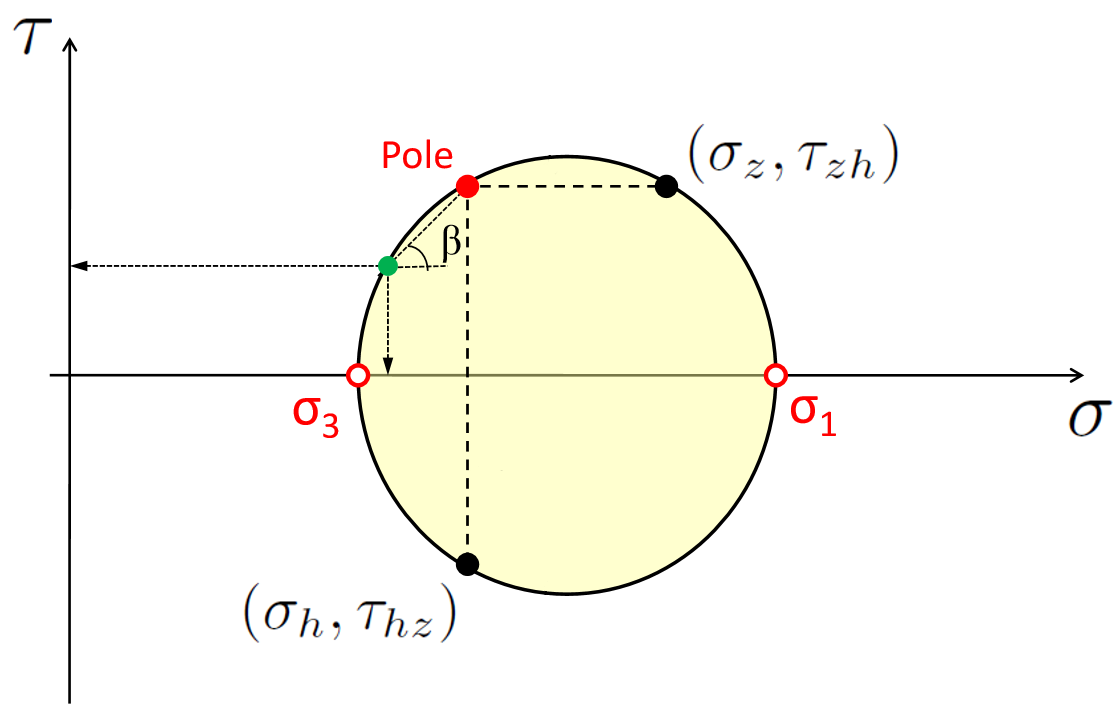
\includegraphics[scale=0.4]{Verastegui/images/V8.PNG}
    \end{multicols}

    \begin{itemize}
        \item La \textbf{contrainte normale} $\sigma$ est positive en compression.
        \item La \textbf{contrainte de cisaillement} $\tau$ est positive si elle produit une rotation antihorlogique.
        \item Le \textbf{cercle de Mohr} à pour but de passer sur tous les états de contraintes applicable à l'échantillon testé.
        \item Le \textbf{pôle} du cercle de Mohr est un point tel qu'une parrallèle tracée par ce point à une facette quelconque recoupe le cercle au point représentatif des contraintes sur cette facette.
        \item La contrainte exercée sur une facette se décompose en une contrainte normale $\sigma$ et une contrainte tangentielle $\tau$. Lorsque seule la contrainte normale est représentée, on l'appelle la \textbf{contrainte principale} majeure et mineure (soit $\sigma_1$ et $ \sigma_3$). Les facettes sur lesquelles elles sont appliquées sont les facettes principales.
        \item Les \textbf{directions principales} sont celles passant par le pôle et les contraintes principales.
        \item Des \textbf{contraintes conjuguées} sont des contraintes parallèles à la facette sur laquelle agit l'autre contrainte. Leur orientation dépend donc de l'orientation de l'autre contrainte sur l'autre facette. 
\end{itemize}
%
%    \subsection{Stress paths}
%    \subsection{Stiffness}
%    \subsection{Shear Modulus}
%    \subsection{Young's Modulus}
%    \subsection{Compression Modulus (bulk modulus)}
%    \subsection{Oedometer Modulus}
    \subsection{Strength}
    
        La force détermine cas de charge extreme qu'un materiaux peu supporter sans rompre. Un matériau rompt lorsque l'effort atteind le rayon maximum de son cercle de Mohr $\tau_f$ 
        
    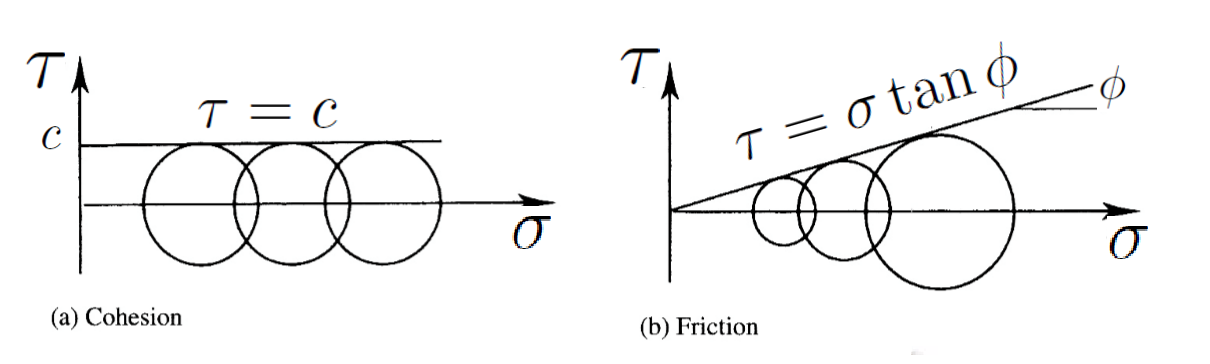
\includegraphics[scale=0.5]{Verastegui/images/V9.PNG} 
        
        il y a deux types de matériau, cohésif et non-cohésif (granulaire)

\section{Shear strength}

    Au plus on augmente l'effort normal sur un sol, au plus il sera difficile de l'amener à rompre. La force de cisaillement dépend de sa densité et de sa quantité de vide ($e$). Ce n'est pas une relation linéaire, mais au plus la densité est élevée, au plus l'est la force.
    
    \begin{figure}[h!]
    \center
    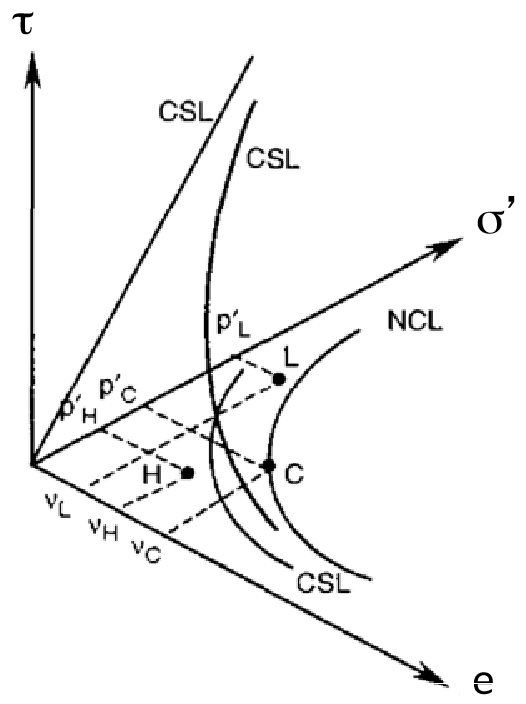
\includegraphics[scale=0.5]{Verastegui/images/V10.PNG}
    \caption{csl = critical state line}
    \end{figure}
    
    \subsection{Drained vs Undrained shear strength of soil}
        \subsubsection{Drained}
        
            \begin{figure}[h!]
            Pour un sol très perméable (sable et gravier) ou pour une charge appliquée très lentement, l'eau à le temps de s'écouler librement. Pendant le cisaillement, le volume va changer, mais il n'y aura pas d'incrémentation de la pression d'eau. La force mise en oeuvre $\tau_f$ est controllée par la force efficace moyenne et le "stress path". Cette force est associée à un volume specifique de rupture $V_f$. Si le volume initial $V_0 \ne V_f$ alors le volume spécifique sera ajusté pour que $V_f$ soit atteind à la rupture. 
            
                \center
                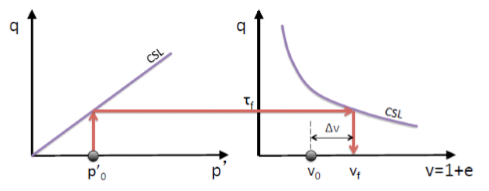
\includegraphics[scale=1]{Verastegui/images/V11.PNG}
            \end{figure}
            
        \subsubsection{Undrained}
        
            \begin{figure}[h!]
            Pour un sol de faible perméabilité (fin limon et argile) ou pour une charge appliquée rapidement, l'eau ne peut se dégager librement. Durant le cisaillement, le volume restera inchangé (et donc également la force efficace moyenne) mais l'excès de pression d'eau peut être mobilisé. La force mise en oeuvre $\tau_f$ est controlée par le volume initial (ou par la densité). cette force est associée à un effort efficace moyen de rupture $P'_f$. Si $P'_0 \ne P'_f$ alors l'effort sera ajusté pour que $p'_f$ soit atteind à la rupture.
    
                \center
                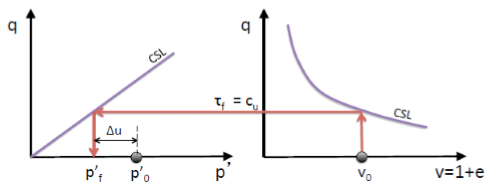
\includegraphics[scale=1]{Verastegui/images/V12.PNG}
            \end{figure}        

    \subsection{Triaxial Compression Test}
        \subsubsection{Consolidated Drained (CD)}
            
            \textbf{$U = 0$} 
            In a consolidated drained test the sample is consolidated and sheared in compression slowly to allow pore pressures built up by the shearing to dissipate. The rate of axial deformation is kept constant, i.e., is strain controlled. The idea is that the test allows the sample and the pore pressures to fully consolidate (i.e., adjust) to the surrounding stresses. The test may take a long time to allow the sample to adjust, in particular low permeability samples need a long time to drain and adjust strain to stress levels.
            
            \begin{figure}[h!]
            \center
                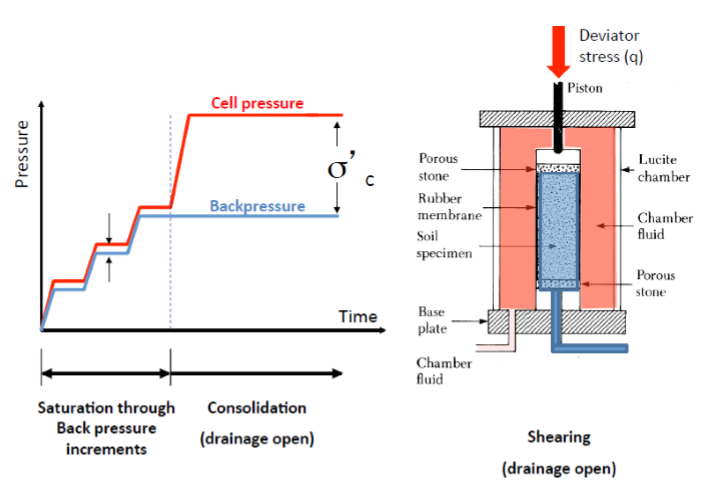
\includegraphics[scale=0.7]{Verastegui/images/V13.PNG}
            \end{figure}     
            
        \subsubsection{Consolidated Undrained (CU)}
        
            \textbf{$U \ne 0$} 
            In a consolidated undrained test the sample is not allow to drain. The shear characteristics are measured under undrained conditions and the sample is assumed to be fully saturated. Measuring the pore pressures in the sample (Sometimes called CUpp) allows approximating the consolidated-drained strength.
            
            \begin{figure}[h!]
            \center
                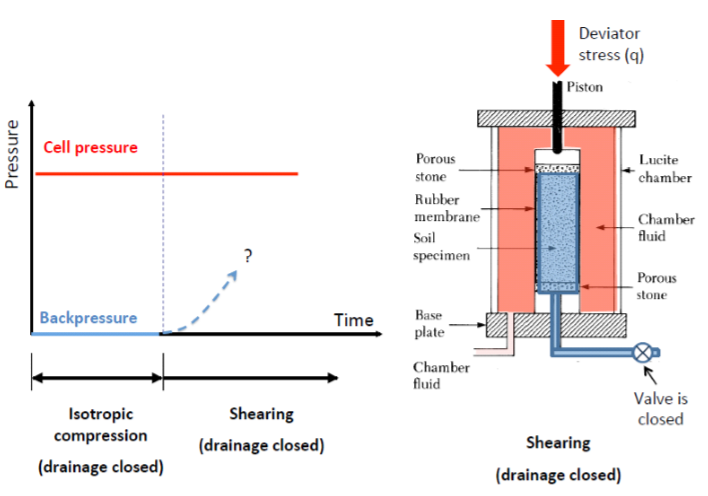
\includegraphics[scale=0.7]{Verastegui/images/V14.PNG}
            \end{figure}
            
        \subsubsection{Unconsolidated Undrained (UU)}
        
            \textbf{$U \ne 0$} 
            In an unconsolidated undrained test the load are applied quickly, and the sample is not allowed to consolidate during the test. The sample is compressed at a constant rate (strain-controlled).
            
            \begin{figure}[h!]
            \center
                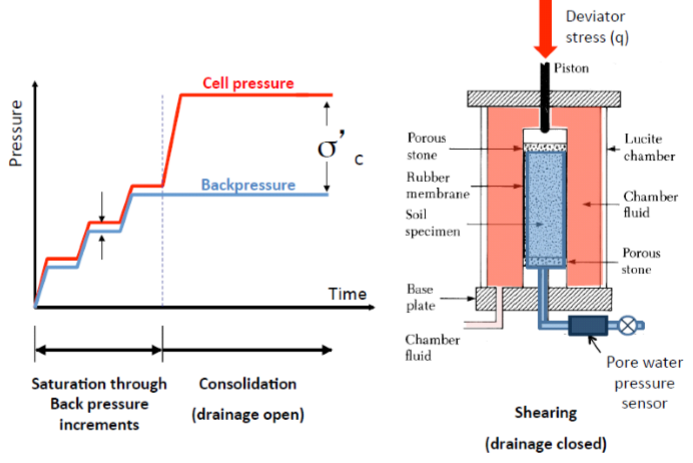
\includegraphics[scale=0.7]{Verastegui/images/V15.PNG}
            \end{figure}
            
        \subsubsection{True Triaxial Test}
        
            Three-axis triaxial testing systems have been developed to allow independent control of the stress in tree perpendicular directions. This allows investigation of stress paths not capable of being generated in axisymetric triaxial test machines, which can be useful in studies of cemented sands and anisotropic soils. the test cell is cubical, and there are six separete plates applying pressure to the specimen, with LVDTs reading movement of each plate. Pressure in the third direction can be applied using hydrostatic pressure in the test chamber, requiring only 4 stress application assemblies. The apparatus is significabtly more complex than for axisymetric triaxial tests, and is therefore less commonly used.
            
\section{Critical State}

\section{Slope Stability}

    Fundamental requirement for stability of slope : "the shear strength of the soil must be greater than the shear stress required for equilibrium." then instability may occur due to a decrease in the shear strength of soil or an increase in the shear stress required for equilibrium.
    
    \medskip
    Some factor could trigger a collapse :
    
    \begin{itemize}
        \item Increase of power water pressure, if $U$ increase then $\sigma'$ decrease and so does the strength (Heavy rainfall).    
        \item Increase of the slope height or the load on the crest. Those factors would increase the shear stresses within the slope.
        \item The liquefaction in the loose soil or any additional shear stress within the slope would lead to a collapse. An earthquake produces that kind of reaction.
    \end{itemize}
    
    \newpage
    \subsection{Limit equilibrium method procedure (3 stages)}
        
        \begin{itemize}
            \item Draw an arbitrary collapse mechanism of slip surfaces : 
                
            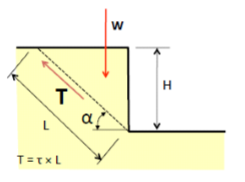
\includegraphics[scale=1]{Verastegui/images/V16.PNG}
        
            \item Resolve the static system of this mechanism by resolving the forces and moments : 
                \medskip
                \begin{center}
                \begin{tabular}{c|c}
                    $\tau = W sin(\frac{\alpha}{L})$  &  $L = \frac{1}{sin \alpha}$  \\
                                                       &  $W = \frac{1}{2} * \gamma * \frac{H^2}{tan \alpha}$ 
                \end{tabular}
                \end{center}
                
            \item Examine the static equilibrium of other mechanisms and find the critical one (the one with a critical loading):
                
                \medskip
                Maximum stress mobilized : $\tau = C_u$, this scenario occurs at $\alpha = 45\degree$. Then with the previous equations : $H_max = \frac{4 C_u}{\gamma}$.
                
            \item Finally we use a factor of safety according to the loads of moments or to the shear strength. 
                
                \medskip
                \begin{center}
                \begin{tabular}{c|c|c}
                    $FS = \frac{S}{\tau}$  
                    &  $FS = \frac{M_{resting}}{M_{driving}}$                        
                    &  $FS = \frac{Stabilising_{Forces}}{Driving_{Forces}}$ 
                \end{tabular}
                \end{center}
        \end{itemize}
        
    \subsection{LEM analysis of infinite slope in drained soil}
    
        % insert shéma
        
        on utilise la définition du facteur de sécurité et de la trigonométrie, 
        
        \begin{multicols}{2}
        
            \begin{flushright}
            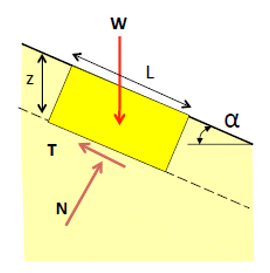
\includegraphics[scale=0.8]{Verastegui/images/V17.PNG}
            \end{flushright}
            
            \vfill\null\columnbreak            
            
            \begin{tabular}{c|c}
                    $FS = \frac{S}{\tau}$ \: &  $\tau = \gamma z \cos \alpha \sin \alpha$  \\
                                             &  $\sigma = \gamma z \cos^2 \alpha$  \\
                                             &  $\sigma' = \gamma z \cos^2 \alpha - u$ 
            \end{tabular} 
            
        \end{multicols}

        on obtient : 
                \begin{center}
                $FS = \frac{c'+(\gamma z \cos^2 \alpha - u) \tan \phi'}{\gamma z \cos \alpha \sin \alpha}$
                \end{center}
                
    \subsection{Method of slice for circular slip surface}
    
        Here, a circular failure surface is assumed and the sliding mass is divided into multiple slices. Static equilibrium of the slice is evaluated. The analysis is repeated for various circular failure surfaces until a most critical failure mechanism is found.
        
        \begin{figure}[h!]
        \begin{multicols}{2}
            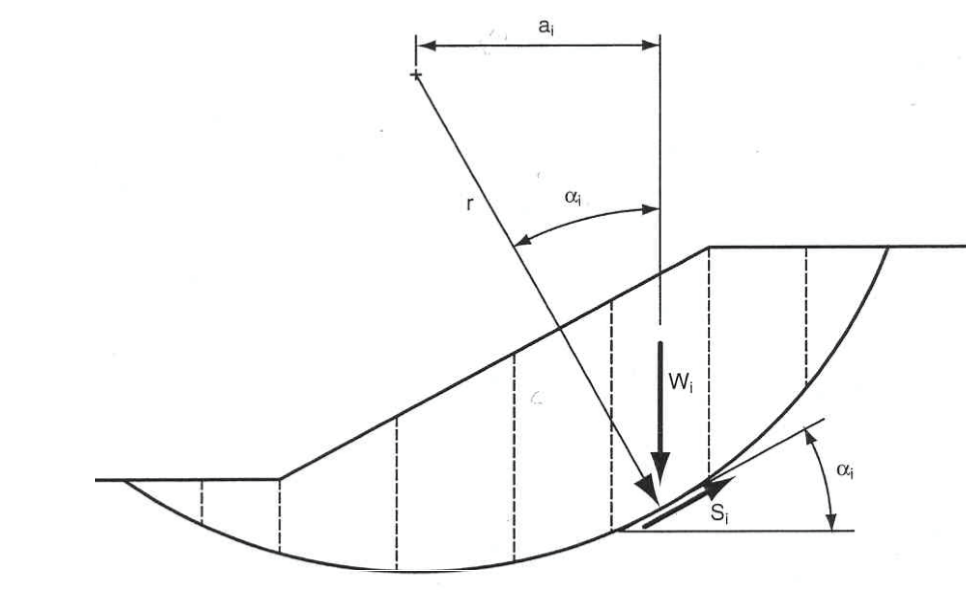
\includegraphics[scale=0.4]{Verastegui/images/V18.PNG}
            \vfill\null\columnbreak
            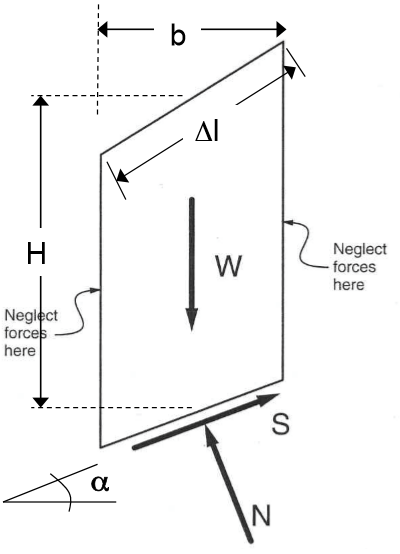
\includegraphics[scale=0.4]{Verastegui/images/V19.PNG}
        \end{multicols}
        \end{figure}
        
        Condition for equilibrium : $M_{drive} = M_{resist}$
        
        \begin{center}
        \begin{itemize}
            \item $M_{drive}$ is due to the self-weight of the slice : $M_{drive} = \sum W_i  a_i = \sum W_i  r \sin \alpha_i$
            \item $M_{resist}$ is due to soil strength : $\sum r S_i = r \sum \tau_i \Delta l_i$
        \end{itemize}
        \end{center}
        
        We can estimate the Security Factor thanks to $\tau_i$ : $FS = \frac{S_i}{\tau_i}$
        By resolving this system we can find an expression for the security factor : 
        
        \begin{center}
        $FS = \frac{\sum (c+\gamma \tan \phi) \Delta l}{\sum W . \sin \alpha}$ 
        \end{center}
        
        The last step is to consider the normal forces : $N = W \cos \alpha$  $\to$ $\sigma = W \frac{\cos \alpha}{\Delta l}$ 
        
        the final equation become : 
        
        \begin{center}
        $FS = \frac{\sum(c' \Delta l + (W.\cos \alpha - u . \Delta l . \cos^2 \alpha) \tan \phi'}{\sum W. \sin \alpha}$
        \end{center}
        
    \subsection{More refined methods}
    
        Some other way to solve the problem exists, such as the GLE, Morgenstren \& Price, Spencer, etc. Those other methods consider interstice forces (normal and shear). As before you have to satisfy the static problem by solving the moment equilibrium problem then satisfy forces equilibrium in both directions. To solve this scenario you have to make somme assumptions :
        
        \begin{itemize}
            \item Spencer : interstice forces are parallel
            \item Morgenstren \& Price : 
                    \begin{tabular}{c|c}
                    $X = f(x) E$  &  $f(x) =$ unknown scalling factor  \\
                                  &  E: Assumed function of known values 
                \end{tabular}
        \end{itemize}
